%!TEX root = ../template.tex
%%%%%%%%%%%%%%%%%%%%%%%%%%%%%%%%%%%%%%%%%%%%%%%%%%%%%%%%%%%%%%%%%%%%
%% chapter3.tex
%% NOVA thesis document file
%%
%% Chapter with a short latex tutorial and examples
%%%%%%%%%%%%%%%%%%%%%%%%%%%%%%%%%%%%%%%%%%%%%%%%%%%%%%%%%%%%%%%%%%%%

\typeout{NT FILE chapter3.tex}%

\chapter{Planning}
\label{cha:planning}
\paragraph{}In this chapter, there will be a description of the work proposal, where the steps needed to complete 
this work will be presented and explained. There will also a schedule with a Gantt Chart showing an estimation of 
the time needed to complete each step and when it will take place. Finaly, there will be a list of potential conferences 
and journals where the results of this work can be published.
\section{Work Proposal}
\label{sec:workproposal}
\paragraph{}To successfully complete this work, there will need to be seven steps. The first step is to create a
simulation model capable of capturing the dynamics of the tractor-trailer system and its environment, here the model of the 
tractor-trailer system will need adaptation as the usual methods of state publishing are not fully equipped to handle passive revolute joints 
like the hitch joint and, to account for this, there is the need to create another method to do so, for example developing a state 
publisher.


The second and third steps are to develop the planning and control algorithms and tune them in the simulator. Some of the 
algorithms and methods mentioned in the previous chapter are implemented in ROS and Gazebo Classic and, to test them in the 
updated ROS 2 and Gazebo Fortress, the algorithms will need to be adapted to the new versions of the software if not completely 
remade. Because of these new conditions, tuning the algorithms will prove to be time consuming and, therefore, a step of 
its own.

The fourth and fifth steps are to implement the algorithms in the real system and test them in a controlled environment. The  
transition from simulation to the real system introduces a new set of challenges to account for, such as sensor imperfections, 
communication delays and errors, and unpredictable environmental events like wind, rain, and also terrain imperfections 
(holes, mud, rocks).

The sixth step is writing the thesis, and the last step is to write a paper with the results of this work and 
publish it in a conference or journal. The publishing of results is categorized as a step of its own as a paper 
will need to be written and the results will also need to be prepared for their presentation.
\clearpage

\begin{figure}[h]
    \centering
    \includegraphics[width=0.9\textwidth]{Proposalarch.png}
    \caption{High level Architecture of the proposed system. The green blocks represent already 
    implemented features, and the pink blocks are the proposed features to be implemented.}
    \label{fig:proposalarch}
\end{figure}

% \clearpage

\section{Schedule}
\label{sec:schedule}
\begin{figure}[h]
    \centering
    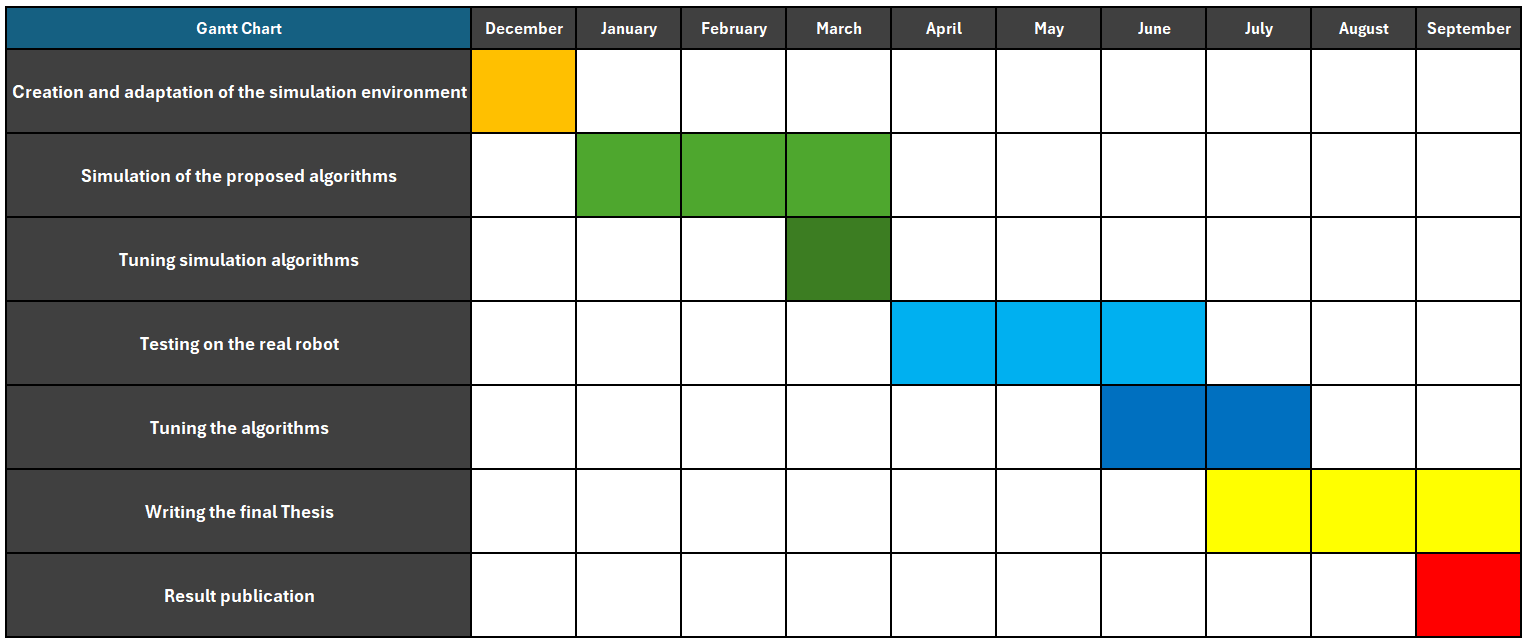
\includegraphics[width=1\textwidth]{ganttV3.png}
    \caption{Gantt Chart with the estimated start time and duration of each of the seven steps needed to finish this work}
    \label{fig:schedule}
\end{figure}
\paragraph{}The schedule for this work is presented in the following Gantt Chart ~\ref{fig:schedule}. 
As mentioned in the previous section, the work is divided into seven steps. 

The adaptation and creation of the simulation environment is estimated to take the month of December. 

The development of the planning and control algorithms is estimated to take the 
three months following, January, February and March with the last month also overlapping with their tuning. 

The implementation of the algorithms in the real system is estimated to take the April, 
May and June, and their tuning will overlap in June and, most likely, extending itself to July. 

While the final adjustments to the system are being make, most of the thesis can be written and, therefore, 
the writing of the thesis will take place from July until its final submission date in September. 

The publication of the results in a conference or journal will depend on how ahead or behind schedule the project is and 
the due date for the first submissions which makes this date very fluid, however, the goal is to have a paper written and published 
by mid August or September. 

Since this document is to be submitted in February, the first and second steps have already been started 
and are currently being worked on. The current approach to the adaptation of the simulation model is to create a 
state publisher which calculates the values of the hitch joint every tenth of a second. The approach may change as the work progresses since it is not fault tolerant and may only be 
a temporary solution to start implementing the planning algorithms, as to not get behind schedule.
In the following figure \ref{fig:publisher} it is possible to see the custom trailer state publisher 
publishing the transforms of the system in Rviz2, on the right, and the simulated state in Gazebo Fortress ,on the left.

\begin{figure}[htbp]
    \centering
    \begin{minipage}[b]{0.4\textwidth}
        \centering
        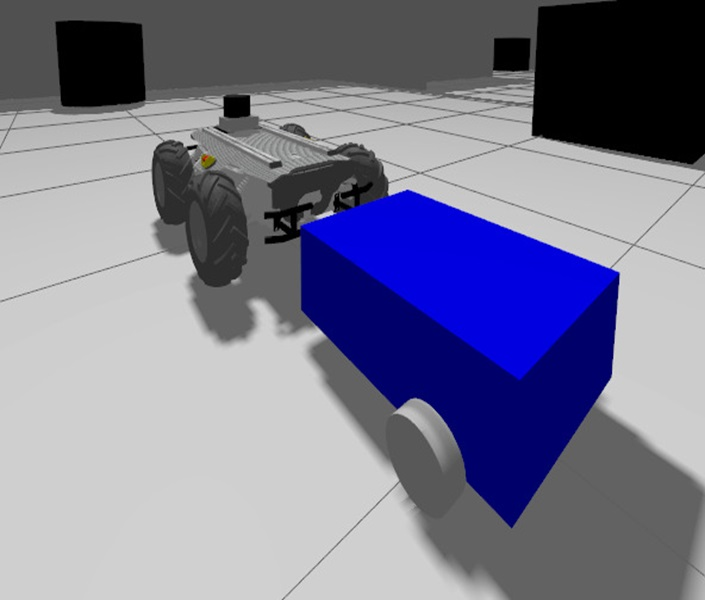
\includegraphics[width=\textwidth]{gazeboSim.jpeg}
    \end{minipage}
    \hspace{0.75cm}
    \begin{minipage}[b]{0.4\textwidth}
        \centering
        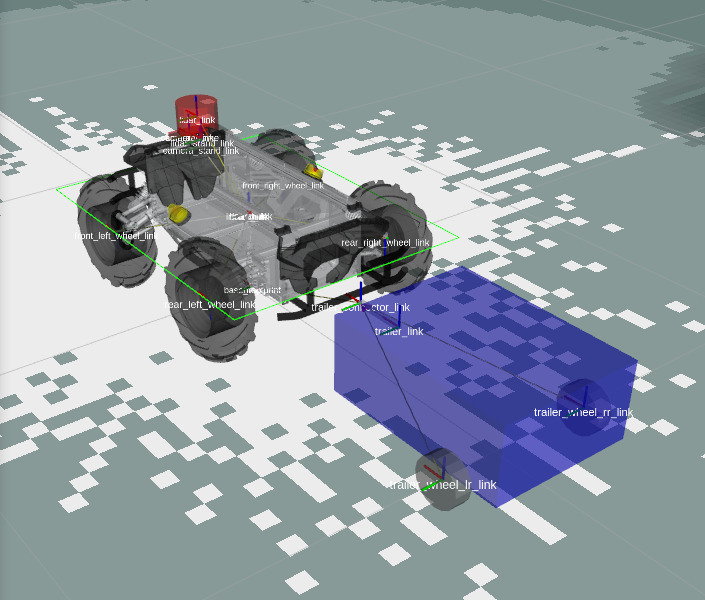
\includegraphics[width=\textwidth]{trailerSim.jpeg} 
    \end{minipage}
    \caption{Gazebo simulation and Rviz2 visualizaton of the current state. The used trailer 
    is an abstraction of the actual trailer, being used for collision detection purposes.}
    \label{fig:publisher}
\end{figure}

The implementation of the planning and control algorithms is also already being worked on, with the current focus 
being the adaptation of the Voronoi algorithm to the new version of ROS.
\clearpage
\section{Results Publishing plan}
\label{sec:resultsplan}
\paragraph{}The results of this work will be published in conferences such as the \textbf{IEEE International Conference on Robotics 
and Automation (ICRA)}, \textbf{IEEE/RSJ International Conference on Mechatronics and Automation (ICMA)}, or the 
\textbf{IEEE International Conference on Intelligent Robots and Systems (IROS)}. These conferences were 
selected because of their focus on robotics, motion planning, and intelligent systems, which are the focus of this project.

The IEEE International Conference on Robotics and Automation is a renowned conference in robotics, 
providing a platform to present research on motion planning and control systems. Its audience includes experts 
in robotics and automation, ensuring that the work is reviewed and discussed by professionals in the field.

The IEEE/RSJ International Conference on Mechatronics and Automation focuses on the integration of mechatronics 
and automation technologies. This conference is relevant for presenting the development and implementation of the 
tractor-trailer system, as it emphasizes the practical application of robotics and control algorithms.

The IEEE International Conference on Intelligent Robots and Systems focuses on intelligent robotics and system 
design. It is well-suited for research involving autonomy and motion planning, making it an appropriate venue for presenting 
the proposed system’s results and findings.

For journal publications, the results will be submitted to \textbf{Expert Systems with Applications}, \textbf{Applied Sciences}, 
or the \textbf{Journal of Intelligent and Robotic Systems}. These journals were chosen for their focus on robotics and intelligent systems, as 
well as their journal score (Q1).

The journal Expert Systems with Applications emphasizes the use of intelligent systems in practical applications. 
It is appropriate for publishing the integration of motion planning and control methods into an agricultural robotics system.

Applied Sciences covers a broad range of engineering topics, including robotics and IoT. It is a good option 
for presenting the varied aspects of this work (motion planning, trailer dynamics, robot control), including its application in precision 
agriculture.

The Journal of Intelligent and Robotic Systems focuses on research in robotics and intelligent systems. It is suitable 
for publishing detailed analyses of the motion planning and control techniques used in this project.

These conferences and journals were chosen to ensure the work reaches a relevant audience and contributes to advancements 
in robotics and precision agriculture. This selection might change as publishing dates for some aren't yet published and may 
not align with the submission of the final dissertation. 